\documentclass{article}
\usepackage[utf8]{inputenc}
\usepackage[spanish]{babel}
\usepackage{csquotes}
\usepackage[backend=bibtex]{biblatex}
\usepackage{hyperref}
\usepackage{graphicx}
\usepackage{amsmath} % Agregado para usar \text{} en las ecuaciones matemáticas

\graphicspath{{./images}}

% Link to the bibliography file
\addbibresource{bibliografia.bib}

\title{Informe Leyes de Newton}
\author{Felipe Colli, Fernando García}
\date{\today}

\begin{document}
\begin{figure}[t]
	\centering % Agregado para centrar el logo si es necesario
	
\includegraphics[width=1\textwidth]{fcfm.jpeg}
\end{figure}

\maketitle
\vspace{1.5cm}

\begin{abstract}
	El presente trabajo expone una revisión introductoria de las tres leyes del movimiento postuladas por Isaac Newton, las cuales constituyen los pilares fundamentales de la mecánica clásica. A través de este documento, se define el concepto de ley científica y se describen los principios de inercia, dinámica (fuerza) y el principio de acción y reacción, acompañados de sus respectivas formulaciones matemáticas. Además, se presentan ejemplos prácticos de la vida cotidiana que ilustran cómo estos principios rigen nuestro entorno físico. Finalmente, se destaca la trascendencia histórica y práctica de las leyes de Newton en el desarrollo tecnológico y en la comprensión de la naturaleza.
\end{abstract}

\newpage
\tableofcontents
\newpage


\section{Introducción}

Desde la antigüedad, el ser humano ha buscado comprender las reglas que gobiernan el movimiento de los cuerpos que lo rodean. Sin embargo, no fue hasta el año 1687 cuando el físico y matemático inglés Isaac Newton publicó su obra cumbre, \textit{Philosophiæ Naturalis Principia Mathematica}, donde sentó las bases de la física moderna. En este histórico texto, Newton formuló tres principios fundamentales que hoy conocemos como las Leyes de Newton, las cuales describen con asombrosa precisión la relación entre las fuerzas que actúan sobre un objeto y el movimiento que este experimenta a velocidades inferiores a la de la luz.

El objetivo de este documento es presentar, de manera clara y estructurada, en qué consisten estas tres leyes: la ley de inercia, la ley de fuerza y la ley de acción y reacción. A lo largo de las siguientes secciones, se abordará la definición conceptual de una ley científica, el significado físico de cada uno de los postulados de Newton y el modelo matemático utilizado para representarlos. Asimismo, para aterrizar estos conceptos teóricos a la realidad, se expondrán diversos ejemplos de la vida cotidiana que evidencian su constante aplicación. De este modo, se busca demostrar la vigencia e importancia de estos principios en el entendimiento de nuestro entorno físico y tecnológico.
\newpage

\


\section{Sobre Leyes de Newton}

\subsection{¿Qué significa la ley?}
Una ley científica es una proposición objetiva, verificada empíricamente, que describe una relación constante y regular entre variables naturales o físicas. Estas leyes, a menudo expresadas matemáticamente, resumen observaciones experimentales repetidas y predicen el comportamiento de la naturaleza bajo condiciones específicas, sin explicar el "porqué" del fenómeno.

\subsection{Qué son las leyes de Newton}
Las leyes de Newton son tres principios fundamentales postulados por Isaac Newton en 1687 que explican la relación entre las fuerzas que actúan sobre un cuerpo y su movimiento. Estas leyes son la base de la mecánica clásica y describen cómo se mueven los objetos cotidianos a velocidades inferiores a la de la luz.

\subsubsection{Ley de inercia}
Un objeto continúa moviéndose con velocidad constante a menos que actúe una fuerza externa. Si el objeto está en reposo, continuará en reposo a menos que actúe una fuerza externa \cite{valdivia_fisica_cap3}. Se dice que un cuerpo está en reposo si la suma de todas las fuerzas que actúan sobre este es igual a 0, es decir, la fuerza neta es 0.

\subsubsection{Ley de Fuerza}
Se define la fuerza como el cambio en el momentum de un cuerpo por el cambio en el tiempo. Se define el momentum como la masa $m$ de un cuerpo multiplicado por su velocidad $\vec{v}$ \cite{nasa_newton_laws}, como se aprecia en la figura \ref{fig:avion_ley_newton}.

La fuerza depende de la masa y la aceleración. A mayor masa, más cuesta acelerar; es decir, se necesita aplicar más fuerza \cite{valdivia_fisica_cap3}.

% Inserta img (Se elimina el entorno center externo, usando solo centering)
\begin{figure}[htbp]
	\centering
	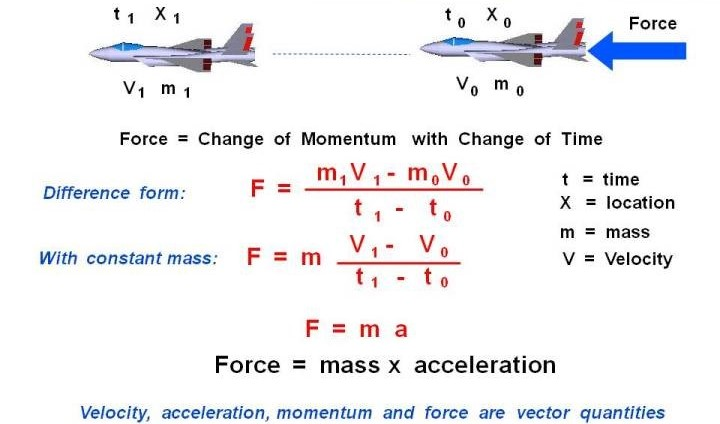
\includegraphics[width=0.8\linewidth]{images/secondlaw.jpg}
	\caption{Segunda Ley de Newton: Relación entre fuerza, masa y aceleración \cite{nasa_newton_laws}}
	\label{fig:avion_ley_newton}
\end{figure}

\subsubsection{Ley de acción y reacción}
A toda acción le corresponde una reacción igual y opuesta. Si el cuerpo A ejerce una fuerza sobre el cuerpo B, el cuerpo B ejerce una fuerza igual y opuesta sobre el cuerpo A.

\subsection{¿Qué ecuaciones se utilizan para modelarlas?}

\subsubsection{Primera ley}
Para la primera ley de Newton usamos:
\[ \sum \vec{F} = 0 \Leftrightarrow \frac{d\vec{v}}{dt} = \vec{0} \]

\subsubsection{Segunda ley}
Para la segunda ley de Newton usamos:
\[ \vec{F} =  m \cdot \vec{a} \quad \text{[N]} \]

\subsubsection{Tercera ley}
Para la tercera ley de Newton usamos:
\[ \vec{F}_{A \rightarrow B} = - \vec{F}_{B \rightarrow A} \]

\subsection{Ejemplos de su aplicación en la vida cotidiana}

\subsubsection{Ley de inercia}
Unos cuantos ejemplos de la ley de la inercia en la vida real son:
\begin{itemize}
	\item Cuando un auto frena de golpe, tu cuerpo se va hacia adelante.
	\item Un cometa en el espacio sigue sin parar siempre y cuando ninguna gravedad le afecte.
	\item Al tirar de un mantel rápidamente, los platos pueden quedarse casi en su lugar.
\end{itemize}

\subsubsection{Ley de fuerza}
Unos cuantos ejemplos de la ley de fuerza en la vida real son:
\begin{itemize}
	\item Empujar un carrito de feria vacío es más fácil que uno con muchas verduras.
	\item Al patear una pelota de fútbol, esta acelera más, y más rápido que al patear una pelota de bolos.
	\item Un avión comercial necesita más motores para poder volar que una avioneta.
\end{itemize}

\subsubsection{Ley de acción y reacción}
Unos cuantos ejemplos de la ley de acción y reacción son:
\begin{itemize}
	\item Al caminar, empujas el suelo hacia atrás y el suelo te impulsa hacia adelante.
	\item El retroceso de un cañón de barco al disparar proyectiles.
	\item Un cohete propulsándose para poder despegar.
\end{itemize}

\newpage

\section{Conclusiones}

Podemos concluir que las leyes de Newton constituyen un trabajo impresionante de Isaac Newton, que nos ha permitido comprender y modelar con gran precisión diversos procesos físicos en la naturaleza. Gracias a estas leyes, es posible explicar el movimiento de los objetos, desde situaciones cotidianas hasta fenómenos más complejos, así como también analizar y desarrollar avances tecnológicos creados por el ser humano, como el funcionamiento de los cohetes y otros sistemas de ingeniería. En este sentido, las leyes de Newton no solo representan un pilar fundamental de la física clásica, sino que también han sido esenciales para el progreso científico y tecnológico a lo largo de la historia.

Un pequeño resumen sobre las leyes de Newton se puede apreciar en el cuadro \ref{tab:tabla_resumen}.

\begin{table}[htbp]
	\centering
	\begin{tabular}{|| l | p{8.5cm} ||}
		\hline
		\textbf{\textit{Ley de Newton}} & \textbf{\textit{Definición}}                                                            \\
		\hline
		Ley de inercia                  & Un objeto no cambia su movimiento (reposo o velocidad) si no actúa una fuerza sobre él. \\
		\hline
		Ley de fuerza                   & $\vec{F} =  m \cdot \vec{a} \quad \text{[N]} $                                          \\
		\hline
		Ley de Acción y Reacción        & A toda acción le corresponde una reacción igual y opuesta.                              \\
		\hline
	\end{tabular}
	\caption{Tabla resumen Leyes de Newton \cite{nasa_newton_laws}}
	\label{tab:tabla_resumen}
\end{table}

\newpage

\printbibliography

\end{document}
